\section{Файлы. Двоичные и текстовые форматы файлов. Файлы прямого и последовательного доступа. Стандартные файлы (потоки)}
\section{Потоки ввода-вывода (C++). Работа с файлами посредством потоков}
\section{Основы объектно-ориентированного программирования: классы, объекты, методы}
\section{Основы объектно-ориентированного программирования: инкапсуляция, наследование, полиморфизм}
\section{Сложность алгоритмов (временнАя и пространственная). Оценки сложности}
\section{Вызов функций (методов). Передача параметров и возврат результата. Рекурсия}
\section{Статическое и динамическое выделение памяти. "Куча"}
\cppref[\textbf{Время хранения}]{cpp/language/storage_duration}~--- это свойство объекта, которое определяет минимальное
возможное время жизни хранилища, содержащего объект.
Время хранения зависит от способа объявления объекта и может быть одним из следующих:

\begin{itemize}
  \itembf{Статическое}. Все глобальные переменные и переменные, впервые объявленные с использованием
  спецификатора \mverb{static} или \mverb{extern}, которые не имеют потоковое время хранения.
  Хранилище живет на протяжении всего исполнения программы. Обычно выделяется в специально отведенном сегменте
  памяти процесса программы~--- сегменте статической памяти (секции \verb|.bss| и \verb|.data|).
  \itembf{Потоковое} {\small\textit{(С C++11)}}. Все переменные, объявленные \mverb{thread_local}.
  Хранилище живет на протяжении жизни потока, в котором переменная создана. У каждого потока имеется
  своя уникальная копия объекта.
  \itembf{Автоматическое}. Смотреть \hyperref[def:auto_storage]{ниже}.
  \itembf{Динамическое}. Все объекты, созданные во время исполнения программы:
  объекты, созданные с помощью оператора \mverb{new} или динамически выделенные на куче,
  а также исключения (которые <<allocated and deallocated in an unspecified way>>).
\end{itemize}

\subsection{Автоматические переменные\footnote{В русскоговорящем сегменте прижилась (несоответствующая стандарту С++) тенденция иногда называть
автоматические переменные статическими (например, \underline{статические} массивы). Следует иметь это в виду; авторы документа придерживаются
исключительно стандарта.}}
Переменная имеет \textbf{автоматическое} время хранения, если выполнено одно из двух условий:
\label{def:auto_storage}
\begin{enumerate}
  \item Переменная принадлежит области видимости блока (\verb|{}|) и явно не объявлена \mverb{static}, \mverb{extern} или \mverb{thread_local}.
  Хранение этих переменных длится до тех пора, пока существует блок, в котором они объявлены.
  \item Переменная является параметром функции. Хранение параметров функции длится до их уничтожения при выходе из функции.
\end{enumerate}
Других автоматических переменных нет.

Автоматические переменные обычно хранятся на стеке, однако компиляторы с целью
оптимизации могут помещать их в регистры процессора. Так или иначе, компилятор обеспечивает их
корректное удаление без дополнительных усилий со стороны программиста.

До C++11 можно было явно указать автоматическое время хранения с помощью
ключевого слова \mverb{auto}. Начиная со стандарта C++11 ключевое слово
\mverb{auto} приобрело новое значение: теперь оно позволяет явно не указывать
тип переменной. В таком случае тип переменной выводится статически во время
компиляции и не может быть изменен во время исполнения.
\begin{minted}{cpp}
std::string ReadName() {
  // автоматическая переменная
  std::string name;
  std::cout << "Введите ваше имя: ";
  std::cin >> name;
  return name;
}

void Welcome(/* автоматическая переменная */
             std::string name1)
{
  std::cout << "Добро пожаловать, " << name1 << "!\n";
} // <- Здесь переменная name1 уничтожена

int main() {
  // автоматическая локальная переменная
  std::string name = ReadName();
  Welcome(name);
} // <- Здесь переменная name уничтожена
\end{minted}

\subsection{Куча}
Отдельным большим сегментом адресного пространства программы выступает куча~--- специальный сегмент памяти для размещения динамических объектов (см. рисунок \ref{fig:memory_segments}).

\begin{figure*}[h]
    \centering
    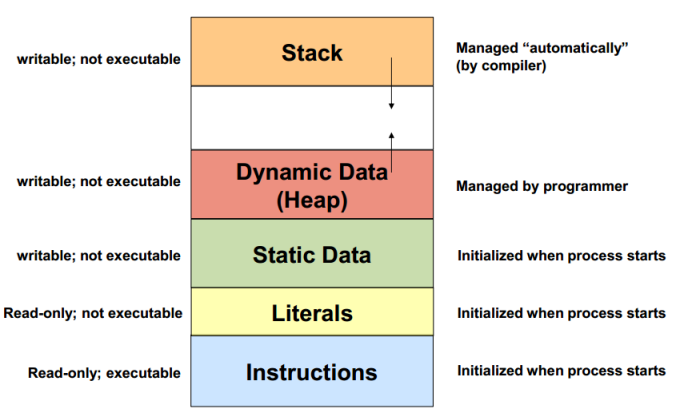
\includegraphics[width=0.5\textwidth]{resources/8-14/mem.png}
    \caption{Сегменты памяти на x86}
    \label{fig:memory_segments}
\end{figure*}

В отличии от сегмента стека, который обычно жестко ограничен и при исчерпании вызывает аварийное завершение программы, объем кучи зависит по в основном
от физически установленной памяти и способности операционной системы в ее предоставлении процессу. Поэтому крупные объекты \textit{практически всегда}
целесообразно размещать именно в куче. Для работы с динамической памятью (т.е. с кучей) в С++ помимо функций языка С
(семейство функций \verb|_alloc()| и \verb|free()|) предоставлены операторы \mverb{new}, \mverb{new[]} и парные им \mverb{delete} и \mverb{delete[]}
соответственно.

Оператор \mverb{new} используется для выделения памяти в куче под один объект одного типа (С С++ 17 можно также указать выравнивание), а оператор
\mverb{new[]} позволяет выделить массив таких объектов\footnote{Особо искушенные последователи Культа
также знают о \cppref[placement new]{cpp/language/new.html\#Placement_new}, который может проинициализировать любой участок памяти (в
т.\,ч. выделенный с помощью \mverb{malloc}). Таким образом можно организовать неинициализированное хранилище под объект (например, при реализации
собственного динамического массива для увеличения скорости)~--- и при том
совершенно легально! Правда, созданные таким образом объекты уничтожить тоже придется вручную, явно вызвав их деструктор.}.

В отличие от языка С, ошибки выделения памяти операторами \mverb{new} и \mverb{new[]} выливаются в выбрасывание исключения \mverb{std::bad_alloc},
которое можно обработать стандартными средствами C++.

% При работе с кучей следует избегать следующих ошибок:
% \begin{itemize}
%     \item Вызов неверной парной функции (например, создание с \mverb{new[]}, а удаление с \mverb{delete}). По стандарту это UB.
%     \item Не вызов \mverb{delete} (\mverb{delete[]}) вовсе. Это называется утечкой памяти.
%     \item Двойной вызов \mverb{delete} (\mverb{delete[]}) на одном и том же участке памяти подряд (double-free). По стандарту это UB.
%     \item Вызов \mverb{delete} (\mverb{delete[]}) на участке памяти, полученном не от оператора \mverb{new} (\mverb{new[]}). Опять же, это UB.
%           В частности, нельзя вызывать \mverb{delete} (\mverb{delete[]}), передавая указатель, полученный от \mverb{malloc()}, даже если вы точно
%           уверены, что (ваш перегруженный) \mverb{new} (\mverb{new[]}) использует его. Для удаления такой памяти есть \mverb{free()}.
% \end{itemize}